\section*{Spectral Dynamics and Information Rates}

Correlation matrices of financial returns fluctuate, and much of econophysics concerns the dynamics of their spectra. Examples include the motion of the market mode, the reshuffling of sector eigenvectors and the alternation of correlation regimes \citep{allez2012eigenvector,munnix2012identifying,schmitt2013non,reigneron2011principal}. The simplest model that has the right symmetries is a symmetric matrix Ornstein--Uhlenbeck process,
\begin{equation}
 \dd H_t=-a\,H_t\,\dd t+\frac1{\sqrt N}\,\dd B_t,
 \label{eq:mou}
\end{equation}
where $B$ is a symmetric matrix Brownian motion whose entries $B_{ij}$, $i<j$, are independent standard Brownian motions and whose diagonal entries are $\sqrt2$ times independent standard Brownian motions. I interpret $H_t$ as the deviation of an $N\times N$ correlation or covariance matrix from its long-run level, with $a>0$ the speed at which correlation shocks dissipate. Matrix-valued diffusions of this kind and their Wishart counterparts have been studied by \citet{bru1991wishart} and \citet{gourieroux2009wishart}. Their eigenvalue dynamics go back to \citet{dyson1962brownian}, and the convergence of their spectra to the semicircle law to \citet{chan1992wigner} and \citet{rogers1993interacting}. The stationary law of \eqref{eq:mou} is the Gaussian orthogonal ensemble scaled so that off-diagonal entries have variance $1/(2aN)$ and diagonal entries $1/(aN)$.

\subsection*{Dyson dynamics and the Burgers equation}

The eigenvalues $\lambda_1(t)>\cdots>\lambda_N(t)$ of $H_t$ satisfy the Dyson system
\begin{equation}
 \dd\lambda_i=\sqrt{\frac2N}\,\dd w_i+\Bigl[\frac1N\sum_{j\neq i}\frac1{\lambda_i-\lambda_j}-a\lambda_i\Bigr]\dd t,
 \label{eq:dyson}
\end{equation}
with independent Brownian motions $w_i$. For the orthogonal symmetry class the eigenvalues never collide after time zero \citep[Section 4.3]{anderson2010introduction}, so \eqref{eq:dyson} has a unique strong solution. The repulsion term is the second-order perturbation of each eigenvalue by the others. The confinement term is the image of the matrix drift, since $-aH$ commutes with every rotation and therefore acts on the spectrum alone. Let $g_t(z)=N^{-1}\tr(z-H_t)^{-1}$. Applying It\^o's formula to $(z-\lambda_i)^{-1}$, symmetrising the repulsion sum through $\sum_{i\ne j}f'(\lambda_i)/(\lambda_i-\lambda_j)=\tfrac12\sum_{i\neq j}[f'(\lambda_i)-f'(\lambda_j)]/(\lambda_i-\lambda_j)$ and noting that the It\^o correction is $O(N^{-1})$, gives in the large-$N$ limit the forced complex Burgers equation
\begin{equation}
 \partial_tg=-g\,\partial_zg+a\,\partial_z(zg).
 \label{eq:burgers}
\end{equation}
The first term is the inviscid Burgers flow of free Brownian motion, whose characteristics are straight lines. In terms of the $R$-transform, it states that the free cumulants of the spectrum increase linearly in time, $R_t(w)=R_0(w)+tw$, which is the free-probability analogue of variance adding under independent increments. The second term is the deterministic contraction. A stationary solution must satisfy $g\,\partial_zg=a\,\partial_z(zg)$. Integrating once and using $g\sim1/z$ at infinity gives $g^2=2a(zg-1)$, so
\[
 g_\infty(z)=az-\sqrt{a^2z^2-2a},\qquad \rho_\infty(x)=\frac1\pi\sqrt{2a-a^2x^2},\quad|x|\le\sqrt{2/a},
\]
the semicircle law of radius $\sqrt{2/a}$. For $a=\tfrac12$ this is the standard semicircle on $[-2,2]$. Started from $H_0=0$, the solution of \eqref{eq:burgers} is at each time a semicircle with variance $\sigma_t^2=(1-e^{-2at})/(2a)$, which interpolates between free Brownian motion at small times and the stationary law. Figure~\ref{fig:dyson} shows a simulated path of the Dyson system for $N=40$ together with the stationary spectrum at $N=400$. The level repulsion visible in the left panel is the mechanism by which sample eigenvalues avoid crossing, and it is the dynamic counterpart of the Marchenko--Pastur spreading.

\begin{figure}[htbp]
\centering
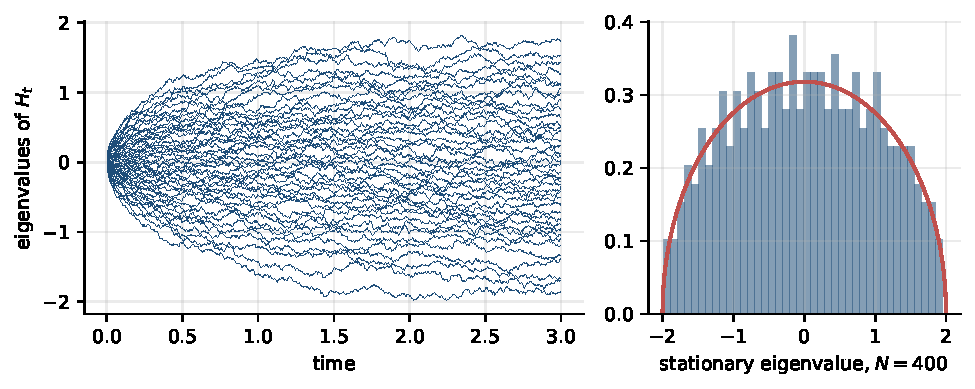
\includegraphics[width=\textwidth]{figures/dyson.pdf}
\caption{Left: eigenvalue trajectories of the matrix Ornstein--Uhlenbeck process \eqref{eq:mou} with $a=\tfrac12$ and $N=40$, started from $H_0=0$ and simulated by Euler steps of length $0.002$. The trajectories repel and never cross. Right: stationary spectrum of a $400\times400$ draw against the semicircle of radius $\sqrt{2/a}=2$, the stationary solution of the Burgers equation \eqref{eq:burgers}.}
\label{fig:dyson}
\end{figure}

\subsection*{Information rates and sufficiency of the spectrum}

Suppose an observer monitors $H$ continuously over $[0,T]$ and must decide whether correlation shocks dissipate at rate $a$ or at rate $b$. Let $P_a^T$ and $P_b^T$ be the corresponding laws of the path $(H_t)_{t\le T}$, both started from the stationary law of the $a$-regime. Let $\Lambda_a^T$ and $\Lambda_b^T$ be the laws of the eigenvalue path $(\lambda(t))_{t\le T}$ alone.

\begin{theorem*}[Information rate and sufficiency of the Dyson process]
For every $N\ge1$ and $T>0$,
\[
 \KL(P_a^T\|P_b^T)=\KL(\Lambda_a^T\|\Lambda_b^T)=T\,\frac{N(N+1)(b-a)^2}{8a}.
\]
Consequently the eigenvector process carries no information about the dissipation rate. By the Chernoff--Stein lemma, the error exponent for discriminating the two regimes from continuous observation is $N(N+1)(b-a)^2/(8a)$ per unit time.
\end{theorem*}

The matrix part is Girsanov's theorem applied to the $N(N+1)/2$ independent coordinates of \eqref{eq:mou} \citep{girsanov1960transforming}. Each off-diagonal coordinate has diffusion variance $1/N$ per unit time and drift difference $(b-a)H_{ij}$. Each diagonal coordinate has diffusion variance $2/N$ and drift difference $(b-a)H_{ii}$. The Kullback--Leibler divergence is half the expected integrated squared drift difference, measured in the inverse diffusion metric:
\[
 \KL(P_a^T\|P_b^T)=\frac N4(b-a)^2\int_0^T\E_a\tr H_t^2\,\dd t,\qquad
 \E_a\tr H_t^2=\frac{N(N-1)}{2aN}+\frac N{aN}=\frac{N+1}{2a}.
\]
The eigenvalue part applies Girsanov's theorem to \eqref{eq:dyson}. The two regimes share the repulsion term and differ only in the confinement, with drift difference $(b-a)\lambda_i$ against diffusion variance $2/N$. This gives $\tfrac N4(b-a)^2\int\E_a\sum_i\lambda_i^2\,\dd t$, which is the same integral because $\sum_i\lambda_i^2=\tr H^2$. The two divergences therefore coincide. Since the eigenvalue path is a measurable function of the matrix path, the data-processing inequality says that equality of divergences is exactly the statement that no information about $a$ is lost by discarding the eigenvectors. The Lean file proves both closed forms and their equality as identities in the field of rationals. The Chernoff--Stein statement is the continuous-time version of the classical result that the optimal type-II error exponent at fixed type-I error equals the Kullback--Leibler rate \citep{chernoff1952measure,cover2006elements}.

Two consequences matter for empirical work. First, the time needed to distinguish two dissipation regimes at a given error level scales as $8a\log(1/\varepsilon)/[N(N+1)(b-a)^2]$. It falls quadratically with the number of assets, because each of the $N(N+1)/2$ independent correlation coordinates contributes its own evidence and rotation invariance concentrates all of that evidence in the $N$ eigenvalues. For $N=10$, $a=\tfrac12$ and $b=1$ the rate is \MOUrate{} nats per unit time, and simulation of the Euler log-likelihood ratio reproduces it in Table~\ref{tab:mc}. Second, the result is a sufficiency statement about a symmetry. If the drift breaks rotation invariance, for example $-a(H-M)$ with a fixed non-scalar target $M$, then the eigenvector process is informative about $M$. The rate for discriminating two targets $M$ and $M'$ at a common $a$ is $\tfrac{a^2N}4\|M-M'\|_F^2$, which includes rotations of $M$ that leave its spectrum unchanged and are therefore invisible to $\lambda(t)$.

The path-space divergence in the theorem is the same object that regularises variational inference for latent stochastic differential equations. There the evidence lower bound subtracts $\tfrac12\E\int\|u_t\|^2\dd t$, with $u$ the recognition drift expressed in the coordinates in which the diffusion is standard \citep{li2020scalable,rice2026sldi}. The sufficiency result therefore has a direct computational corollary for matrix-valued latent states. If both the generative and the recognition drifts are rotation-equivariant spectral functions of $H$, the Kullback--Leibler term and the likelihood of any rotation-invariant observation depend on the eigenvalue path alone. Variational inference can then be carried out on the $N$-dimensional Dyson system rather than on the $N(N+1)/2$ matrix coordinates, without loss. At a finite time step $\Delta$, the Euler transition laws under the two regimes share their Gaussian covariance and differ only in their means. The chain rule for relative entropy therefore gives a per-step divergence of $\tfrac N4(b-a)^2\Delta\tr H^2$ at the current state, both for the matrix chain and, with $\sum_i\lambda_i^2$ in place of $\tr H^2$, for the eigenvalue chain. The two discrete rates agree up to the $O(\Delta)$ discrepancy between the stationary second moments of the two Euler chains. The stationary initial laws contribute an additional, horizon-independent divergence of $\tfrac{N(N+1)}4[b/a-1-\log(b/a)]$ when the two regimes are started from their own stationary laws. Because this term grows like $N^2$ as well, cross-sectional information about correlation regimes is abundant both in snapshots and in dynamics.
